\documentclass[12pt]{article}

% \usepackage[default]{sourcecodepro}
% \usepackage[T1]{fontenc}

\usepackage{amsfonts, lipsum}
\usepackage{amsmath,amssymb, amscd,amsbsy, bbm, amsthm, enumerate}
\usepackage{mdframed, titlesec, setspace,verbatim, multicol}
\usepackage[top=1in, bottom=1in, left=.45in, right=.45in]{geometry}
\usepackage[unicode]{hyperref}
\usepackage{tikz, pgfplots, xcolor, fancyhdr}
\usepackage{graphicx, caption, subcaption}
\usepackage{stmaryrd}

\setlength{\parindent}{0pt}
\setlength{\textheight}{9in}

%%% Header and Footer Info
\pagestyle{fancy}
% \fancyhead[L]{{\large CSE431 Assignment 4}}
% \fancyhead[C]{}
% \fancyhead[R]{Name: Bradley Bauer}
\fancyhead[L]{\large CSE 431 Assignment 4 }
\fancyhead[C]{}
\fancyhead[R]{\large Question 3}

\theoremstyle{definition}

%%% These are some shortcuts that are handy
\def\real{{\mathbb R}}
\def\Natural{\mathbb{N}}
\def\dx{\textnormal{dx}}
\def\dy{\textnormal{dy}}
\def\dz{\textnormal{dz}}
\def\dt{\textnormal{dt}}
\def\ds{\textnormal{ds}}
\def\dw{\textnormal{dw}}
\def\Re{\textnormal{Re}}
\def\Im{\textnormal{Im}}
\def\exp{\textnormal{exp}}
\def\interior{\textnormal{interior}}
\def\al{\alpha}
\def\del{\delta}
\def\Del{\Delta}
\def\gam{\gamma}
\def\Gam{\Gamma}
\def\Om{\Omega}
\def\ep{\varepsilon}
\def\lam{\lambda}
\def\rational{{\mathbb Q}}
\def\integer{{\mathbb Z}}
\def\Q{{\mathbb Q}}
\def\Z{{\mathbb Z}}
\def\N{{\mathbb N}}
\def\R{{\mathbb R}}
\def\grad{\nabla}
\def\C{\mathcal C}
\def\P{\mathcal P}
\def\T{\mathcal T}
\def\I{\mathcal I}
\newcommand{\abs}[1]{\left| #1 \right|}
\newcommand{\inner}[1]{\langle #1 \rangle}
\newcommand{\norm}[1]{\left\lVert#1\right\rVert}
\newcommand{\spanvect}{\textnormal{span}}
\newcommand{\union}{\cup}
\newcommand{\Union}{\bigcup}
\def\intersect{\cap}
\def\Intersect{\bigcap}

\newtheorem{innercustomthm}{}
\newenvironment{question}[1]
  {\renewcommand\theinnercustomthm{#1}\innercustomthm}
  {\endinnercustomthm}

\begin{document}

\begin{question}{Hypothesis}
    I expect the hashtable to be a lot faster than the binary tree.
\end{question}

\begin{question}{Methods}
    The experiment is ran on Ubuntu 19.04. GCC version is 8.3 and python version is 3.7.3.
    Also, matplotlib, pandas, and numpy are dependencies of plot.py\\\\
    To run the experiment, first compile
    $$\text{g++ -fconcepts -std=c++2a -O3 code.cpp}$$
    Then execute $$\text{./a.out}$$
    which may take a few minutes to run.
    To plot the results use
    $$\text{python3 plot.py}$$
    The program compares binary tree and hash table insertion performance for various input sizes n in the range [0, 4466816].
    For each input size n, the program inserts n uniform random integers into a binary tree and into a hash table.
    The total time taken for inserting n elements into the binary tree is recorded and similarly for the hashtable.
\end{question}

\newpage
\begin{question}{Results}
$\\$
\vspace{-1cm}
\begin{figure}[h]
  \centering
  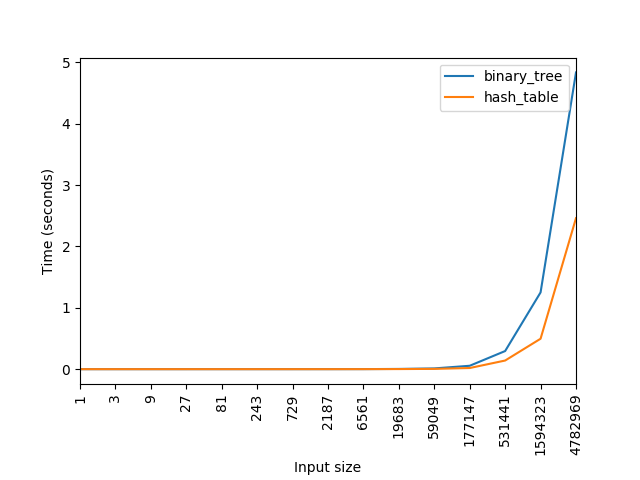
\includegraphics[width=\textwidth]{Figure_1.png}
  \caption{}
  \label{fig:boat1}
\end{figure}

\begin{figure}[h]
  \centering
  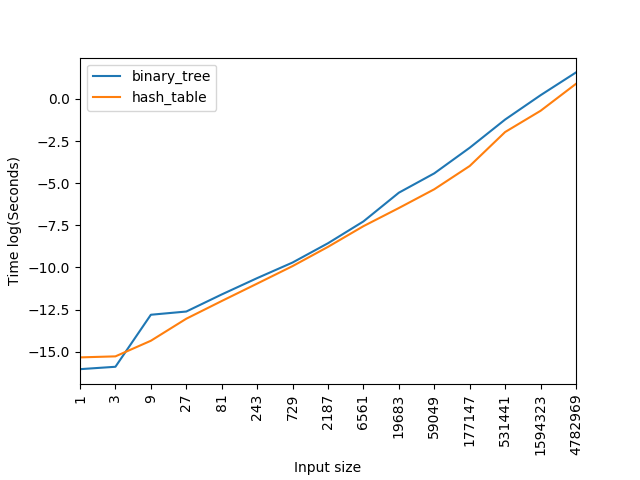
\includegraphics[width=\textwidth]{Figure_2.png}
  \caption{}
  \label{fig:boat2}
\end{figure}

Figure 1 simply gives the time to insert n items vs the value for n.
\newpage
Figure 2 shows the same data as in Figure 1 but with a log scale n the vertical axis.

\end{question}

\begin{question}{Discussion}
  From the plots we can see that the binary tree is competitive with the hash table for input sizes of 10000 or less.
\end{question}

\begin{question}{Conclusion}
  Binary trees are competitive with hash tables for input sizes of 10000 or less.
\end{question}

\end{document}
